\label{sec:compressore}
\section{Compressore}

Il compressore è stato modellato come una turbomacchina assiale adiabatica finalizzata ad incrementare la pressione totale del fluido prima dell'ingresso nella camera di combustione.

La trasformazione è stata descritta mediante un rendimento politropico costante ($\eta_{p,c}=0.90$), dal quale è stato ricavato il corrispondente rendimento isoentropico. Le prestazioni termodinamiche, il dimensionamento geometrico e le verifiche aerodinamiche sono riportati in Appendice~\ref{app:compressore}.

\subsection{Primo stadio del compressore}


%La velocità periferica di punta $U_{tip}$ è ottenuta dall'ottimizzazione. In una prima stima viene imposto un fattore di De Haller pari a $0.72$, dal quale si ricava il lavoro specifico teorico per stadio e quindi il numero di stadi richiesto. Poiché tale numero deve essere intero, viene arrotondato per eccesso e il triangolo di velocità viene successivamente ricalcolato distribuendo il lavoro complessivo sul numero effettivo di stadi. Il fattore di De Haller finale risulta quindi leggermente superiore al valore imposto inizialmente. Nel punto di progetto si ottiene infatti $DeHaller=0.7296$.

%----------------------

Il dimensionamento è stato effettuato al raggio medio assumendo
$V_a=\mathrm{cost}$ e ingresso
assiale nel primo rotore ($V_{\theta,1}=0$). La geometria anulare di
ingresso è stata definita imponendo un rapporto mozzo-punta
$r_{h,2}/r_{t,2}=0.5$, mentre lungo il compressore è stato mantenuto
costante il raggio di punta.

Il numero di stadi è stato stimato mediante l'approssimazione a stadi
ripetuti. Lo statore è considerato privo di lavoro meccanico e riporta
il flusso alle condizioni richieste all'ingresso dello stadio successivo.
La velocità periferica di punta $U_{tip}$ è ottenuta dall'ottimizzazione.
In una prima stima viene imposto un fattore di De Haller pari a $0.72$,
dal quale si ricava il lavoro specifico teorico per stadio. Il numero di
stadi viene quindi arrotondato per eccesso e il triangolo di velocità
ricalcolato distribuendo il lavoro complessivo sul numero intero di
stadi ottenuto. Nel punto di progetto risulta $DeHaller=0.730$.

Per le verifiche aerodinamiche sono state assunte solidità
$\sigma_r=1.0$ per il rotore e $\sigma_s=1.25$ per lo statore.
La corda e il numero di pale rotoriche sono stati determinati imponendo
$Re_c\geq3\times10^5$.

%--------------------------------
%\begin{figure}[H]
%    \centering
%    \includegraphics[width=0.75\textwidth]
%    {Graphics/turbogetto/compressore/triangoli_compressore_immagine3.png}
%    
%    \caption{Triangoli di velocità all'ingresso e all'uscita del rotore del primo stadio del compressore.}
%    \label{fig:compressore:triangoli}
%\end{figure}

% Pala con profilo NACA 2412 approssimato.
% Uso: \DrawBlade{x}{y}{angolo}

\newcommand{\DrawBlade}[3]{%
  \begin{scope}[shift={(#1,#2)},rotate=#3,xscale=2.2,yscale=2.2]

    % Profilo della pala di turbina (curvatura a C)
    \draw[thick,fill=gray!10,line join=round]
      % Estradosso (suzione - molto convesso)
      plot[smooth] coordinates {
        (0.000, 0.000)
        (0.050, 0.120)
        (0.150, 0.220)
        (0.300, 0.280)
        (0.450, 0.270)
        (0.600, 0.220)
        (0.750, 0.140)
        (0.900, 0.060)
        (1.000, 0.000)
      }
      --
      % Intradosso (pressione - nettamente concavo)
      plot[smooth] coordinates {
        (1.000, 0.000)
        (0.850, 0.040)
        (0.700, 0.080)
        (0.550, 0.120)
        (0.400, 0.140)
        (0.250, 0.130)
        (0.120, 0.080)
        (0.050, 0.030)
        (0.000, 0.000)
      }
      -- cycle;

    % Linea media (Camber line)
    \draw[dashed,gray!65,thin]
      plot[smooth] coordinates {
        (0.000, 0.000)
        (0.150, 0.150)
        (0.350, 0.210)
        (0.600, 0.170)
        (0.800, 0.090)
        (1.000, 0.000)
      };

  \end{scope}%
}


% ============================================================
% PARAMETRI MODIFICABILI
% ============================================================
\def\Denom{50}

% Pale
\def\BladeAngle{105}
\def\BladeY{-6.8}

% Triangolo di ingresso
\def\OoneX{0}
\def\OoneY{0}

% Estremo di V1
% VoneX diverso da OoneX rende V1 inclinato.
\def\VoneX{0/\Denom}
\def\VoneY{-154/\Denom}

% Estremo di W1
\def\WoneX{-248/\Denom}
\def\WoneY{-154/\Denom}

% Valori visualizzati
\def\VoneValue{154}
\def\WoneValue{292}
\def\UoneValue{248}

% Angoli visualizzati
\pgfmathsetmacro{\AlphaOneValue}{round(10*atan2(abs(\VoneX),abs(\VoneY)))/10}
\def\BetaOneValue{58.1}

% Triangolo di uscita
\def\OtwoX{9}
\def\OtwoY{\BladeY-1}

% Estremo di V2
\def\VtwoX{101/\Denom+\OtwoX}
\def\VtwoY{-154/\Denom+\OtwoY}

% Estremo di W2
\def\WtwoX{-147/\Denom+\OtwoX}
\def\WtwoY{-154/\Denom+\OtwoY}

% Valori visualizzati
\def\VtwoValue{184}
\def\WtwoValue{213}
\def\UtwoValue{248}

% Angoli visualizzati
\def\AlphaTwoValue{33.3}
\def\BetaTwoValue{43.6}



\begin{figure}[H]
\centering
\begin{tikzpicture}[
  scale=0.8,
  font=\fontsize{7}{8}\selectfont,
  absolute/.style={ultra thick,cyan!80!blue,-{Stealth[length=3mm,width=2.2mm]}},
  relative/.style={ultra thick,orange,-{Stealth[length=3mm,width=2.2mm]}},
  peripheral/.style={ultra thick,green!70!black,-{Stealth[length=3mm,width=2.2mm]}},
  reference/.style={dashed,gray!60,thin},
  velocitylabel/.style={text=black,fill=white,inner sep=2pt},
  angletext/.style={text=black,fill=white,inner sep=1pt}
]

% ============================================================
% TRIANGOLO DI INGRESSO
% ============================================================

\coordinate (O1) at (\OoneX,\OoneY);
\coordinate (V1) at (\VoneX,\VoneY);
\coordinate (W1) at (\WoneX,\WoneY);
\coordinate (VerticalOne) at (\OoneX,-3.1);

% Linea verticale di riferimento
\draw[reference] (O1) -- (VerticalOne);

% Vettore V1
\draw[absolute]
  (O1) -- (V1)
  node[velocitylabel,midway,right=2pt]
  {$v_{1}=\VoneValue\,\mathrm{m/s}$};

% Vettore W1
\draw[relative]
  (O1) -- (W1)
  node[velocitylabel,midway,below left=1pt]
  {$w_{1}=\WoneValue\,\mathrm{m/s}$};

% Vettore U1
\draw[peripheral]
  (W1) -- (V1)
  node[velocitylabel,midway,below=5pt]
  {$U=\UoneValue\,\mathrm{m/s}$};

% Arco beta 1
\pic[
  draw,
  angle radius=1.25cm
]
  {angle=W1--O1--VerticalOne};

\node[angletext]
  at (1,-0.7)
  {$\beta_1=\BetaOneValue^\circ$};

% Arco alpha 1
% Diventa visibile quando V1 viene inclinato.
%\pic[
%  draw,
%  angle radius=0.72cm
%]
%  {angle=VerticalOne--O1--V1};

%\node[angletext]
%  at (1.6,0)
%  {$\alpha_{1.5} = \pgfmathprintnumber[fixed, precision=1]{\AlphaOneValue}^\circ$}


% ============================================================
% PALE NACA
% ============================================================

\DrawBlade{0}{\BladeY}{\BladeAngle}
\DrawBlade{2}{\BladeY}{\BladeAngle}
\DrawBlade{4}{\BladeY}{\BladeAngle}
\DrawBlade{6}{\BladeY}{\BladeAngle}
\DrawBlade{8}{\BladeY}{\BladeAngle}




% ============================================================
% FRECCIA DI ROTAZIONE
% ============================================================

\node[
  single arrow,
  draw=green!70!black,
  fill=white,
  thick,
  minimum height=1cm,
  minimum width=0.5cm,
  single arrow head extend=0.1cm,
  anchor=east,
  shape border rotate=0
]
  (rotor) at (-1,\BladeY+1) {};

\node[
  left=4pt,
  align=center,
  font=\sffamily\scriptsize
]
  at (rotor.west)
  {\textbf{Rotazione}\\\textbf{del rotore}};


% ============================================================
% PIANO DI USCITA
% ============================================================

\draw[gray!65,thin]
  (-1,\BladeY) -- (9,\BladeY);

\node[below,text=gray!65,font=\scriptsize]
  at (3.2,\BladeY)
  {piano di uscita del rotore};


% ============================================================
% TRIANGOLO DI USCITA
% ============================================================

\coordinate (O2) at (\OtwoX,\OtwoY);
\coordinate (V2) at (\VtwoX,\VtwoY);
\coordinate (W2) at (\WtwoX,\WtwoY);
\coordinate (VerticalTwo) at (\OtwoX,\BladeY-4);

% Linea verticale di riferimento
\draw[reference] (O2) -- (VerticalTwo);

% Vettore V2
\draw[absolute]
  (O2) -- (V2)
  node[velocitylabel,midway,below right=2pt]
  {$v_2=\VtwoValue\,\mathrm{m/s}$};

% Vettore W2
\draw[relative]
  (O2) -- (W2)
  node[velocitylabel,midway,left=10pt]
  {$w_2=\WtwoValue\,\mathrm{m/s}$};

% Vettore U2
\draw[peripheral]
  (W2) -- (V2)
  node[velocitylabel,midway,below=8pt]
  {$U=\UtwoValue\,\mathrm{m/s}$};

% Arco alpha 2
\pic[
  draw,
  angle radius=0.6cm
]
  {angle=VerticalTwo--O2--V2};

\node[angletext]
  at (10.4,\BladeY-1.5)
  {$\alpha_2=\AlphaTwoValue^\circ$};

% Arco beta 2
\pic[
  draw,
  angle radius=1cm
]
  {angle=W2--O2--VerticalTwo};

\node[angletext]
  at (8.2,\BladeY-3)
  {$\beta_2=\BetaTwoValue^\circ$};



\draw[->, thick] (9,0) -- (10.5, 0) node[right] {$\theta$};
% Asse theta (verticale)
\draw[->, thick] (9,0) -- (9, -1.5) node[below] {$z$};
% Origine
\fill (0,0) circle (1.5pt);

  
\end{tikzpicture}
    \caption{Triangoli di velocità all'ingresso e all'uscita del rotore del primo stadio del compressore.}
    \label{fig:compressore:triangoli}
\end{figure}




%------------------------

\begin{figure}[H]
    \centering

    %---------------------------------------------------------
    % MINIPAGE SINISTRA: rappresentazione grafica
    %---------------------------------------------------------
    \begin{minipage}[c]{0.50\textwidth}
        \centering
        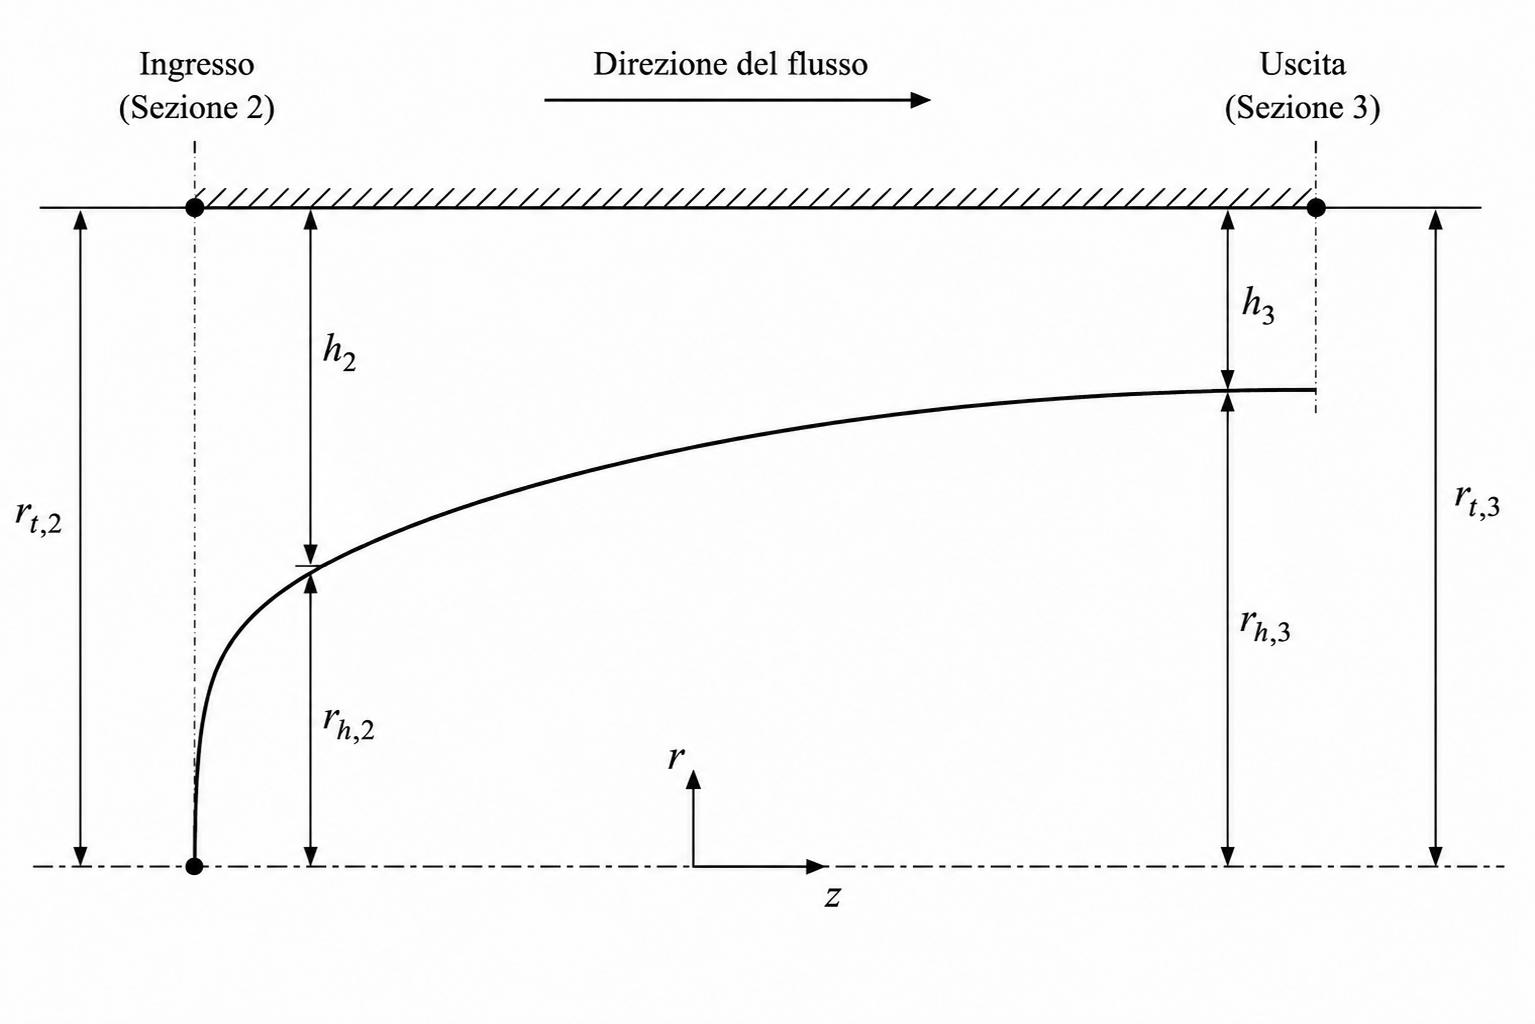
\includegraphics[width=\linewidth]
        {Graphics/turbogetto/compressore/schema_compressore.png}
    \end{minipage}%
    \hfill
    %---------------------------------------------------------
    % MINIPAGE DESTRA: tabella
    %---------------------------------------------------------
\begin{minipage}[c]{0.34\textwidth}
    \centering

    \footnotesize
    \fontsize{11pt}{11pt}\selectfont
    \renewcommand{\arraystretch}{1}
    \setlength{\tabcolsep}{3pt}

    \begin{tabular}{lc}
        \toprule
        \textbf{Dimensione} & \textbf{Valore [mm]} \\
        \midrule

        $r_{t,2}$ & 500 \\
        $r_{h,2}$ & 250 \\
        $r_{m,2}$ & 375 \\
        $h_2$     & 250 \\

        \addlinespace

        $r_{t,3}$ & 500 \\
        $r_{h,3}$ & 470 \\
        $r_{m,3}$ & 485 \\
        $h_3$     & 30.0 \\

        \bottomrule
    \end{tabular}
\end{minipage}

    \caption{Geometria del canale anulare del compressore e principali
    dimensioni nelle sezioni di ingresso e di uscita.}
    \label{fig:geometria_compressore}
\end{figure}

%---------------------------------
\begin{table}[H]
    \centering
    \caption{Principali parametri del compressore.}
    \label{tab:compressore_risultati}
    \fontsize{11pt}{11pt}\selectfont
    \renewcommand{\arraystretch}{1}
    \begin{tabular}{lcccc}
        \toprule
        \textbf{Grandezza} &
        \textbf{Simbolo} &
        \textbf{Valore} &
        \textbf{Limite} &
        \textbf{Unità} \\
        \midrule

        Rapporto di compressione
        & $\pi_c$ & 13.8 & -- & -- \\

        Rendimento politropico
        & $\eta_{p,c}$ & 0.900 & -- & -- \\

        Rendimento isoentropico
        & $\eta_c$ & 0.859 & -- & -- \\

        Potenza assorbita
        & $\dot{L}_c$ & 10.8 & -- & MW \\

        Velocità periferica di punta
        & $U_{tip}$ & 330 & -- & m/s \\

        Numero di stadi
        & $N_{\mathrm{stadi}}$ & 13 & $<15$ & -- \\

        Numero di pale rotoriche
        & $N_{\mathrm{pale,r}}$ & 50 & -- & -- \\

        \midrule

        Mach relativo massimo
        & $M_{\mathrm{rel}}$ & 0.946 & $<1$ & -- \\

        Fattore di De Haller
        & $DeHaller$ & 0.730 & $>0.72$ & -- \\

        Coefficiente di carico
        & $C_p$ & 0.468 & $<0.5$ & -- \\

        Coefficiente di diffusione rotore
        & $D_r$ & 0.443 & $<0.6$ & -- \\

        Coefficiente di diffusione statore
        & $D_s$ & 0.383 & $<0.6$ & -- \\

        Grado di reazione
        & $R$ & 0.796 & -- & -- \\

        \bottomrule
    \end{tabular}
\end{table}



%----------------
I risultati ottenuti rispettano i vincoli aerodinamici e geometrici
introdotti nell'ottimizzazione, in modo particolare il compressore presenta un rapporto di compressione
$\pi_c=13.8$ e richiede 13 stadi.























